\chapter{PENGUJIAN DAN EVALUASI}
\tab Pengujian dilakukan untuk memastikan kualitas perangkat lunak yang dikembangkan dan kesesuaian hasil eksekusi perangkat lunak dengan analisis dan perancangan perangkat lunak.

\section{Tujuan Pengujian}
\tab Pengujian dilakukan terhadap sistem easymeeting guna mengetahui
beberapa hal berikut:
\begin{enumerate}
	\item Menguji kesesuaian dan ketepatan fungsionalitas dari seluruh sistem aplikasi.
	\item Menguji kesesuaian \textit{tools} yang digunakan dalam pengembangan sistem easymeeting.
\end{enumerate}

\section{Kriteria Pengujian}
\tab Penilaian atas pencapaian tujuan pengujian didapatkan dengan memperhatikan beberapa hasil yang diharapkan berikut ini:
	\begin{enumerate}
	\item Kemampuan sistem untuk menyalakan dan memadamkan lampu.
	\item Kemampuan sistem untuk menyalakan dan memadamkan AC.
	\item Kemampuan sistem untuk menampilkan status kondisi lampu dan AC ruangan.
	\item Kemampuan sistem untuk menampilkan suhu ruangan.
	\item Kemampuan sistem untuk diimplementasikan dengan menggunakan WSO2 IoT Server.
	\end{enumerate}

\section{Skenario Pengujian}
\tab Skenario pengujian dilakukan dengan melakukan peran sebagai pegawai yang akan melakukan rapat di ruangan dalam gedung yang akan menyiapkan ruang rapat tersebut melalui Telegram. Dalam skenario ini pegawai diasumsikan telah menambahkan bot easymeeting dalam kontak aplikasi Telegram-nya. Langkah-langkah dari skenario untuk penjual adalah berikut ini :
	\begin{enumerate}
		\item Pegawai membuka aplikasi Telegram.
		\item Pegawai membuka bot easymeeting pada aplikasi Telegram.
		\item Pegawai mengirimkan perintah "/start" kepada Bot Telegram untuk menampilkan perintah yang tersedia pada Bot.
		\item Pegawai mengirimkan perintah "/kontrol" kepada Bot Telegram untuk menampilkan menu dengan tampilan GUI pada Telegram.
		\item Pegawai mengirimkan perintah "/status" untuk menampilkan kondisi Lampu dan AC pada ruang rapat.
		\item Pegawai mengirimkan perintah "/nyalakan" dan "/matikan" melalui menu GUI yang tersedia pada Telegram untuk menyiapkan lampu dan AC dalam ruang rapat.
		\item Skenario selesai.
	\end{enumerate}
	
\section{Evaluasi Pengujian}
\tab Hasil pengujian dilakukan terhadap pengamatan mengenai perilaku easymeeting terhadap kasus skenario uji coba. Pengujian dilakukan dari pihak developer dan pembimbing lapangan.
\begin{figure}[H]
	\centerline {
		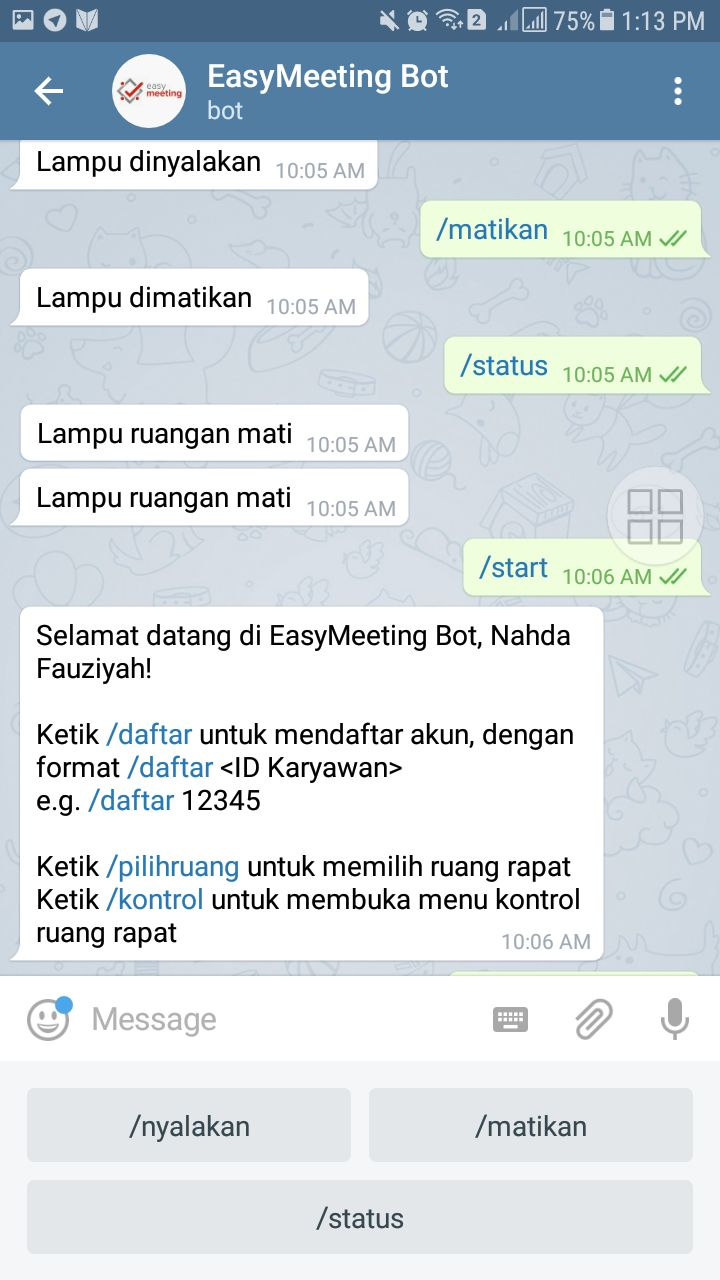
\includegraphics[width=3.5cm]{bab6/img/start.jpeg}
	}
	\caption{Mengirimkan Perintah "/start"}
	\label{figure:start}
\end{figure}
\begin{figure}[H]
	\centerline {
		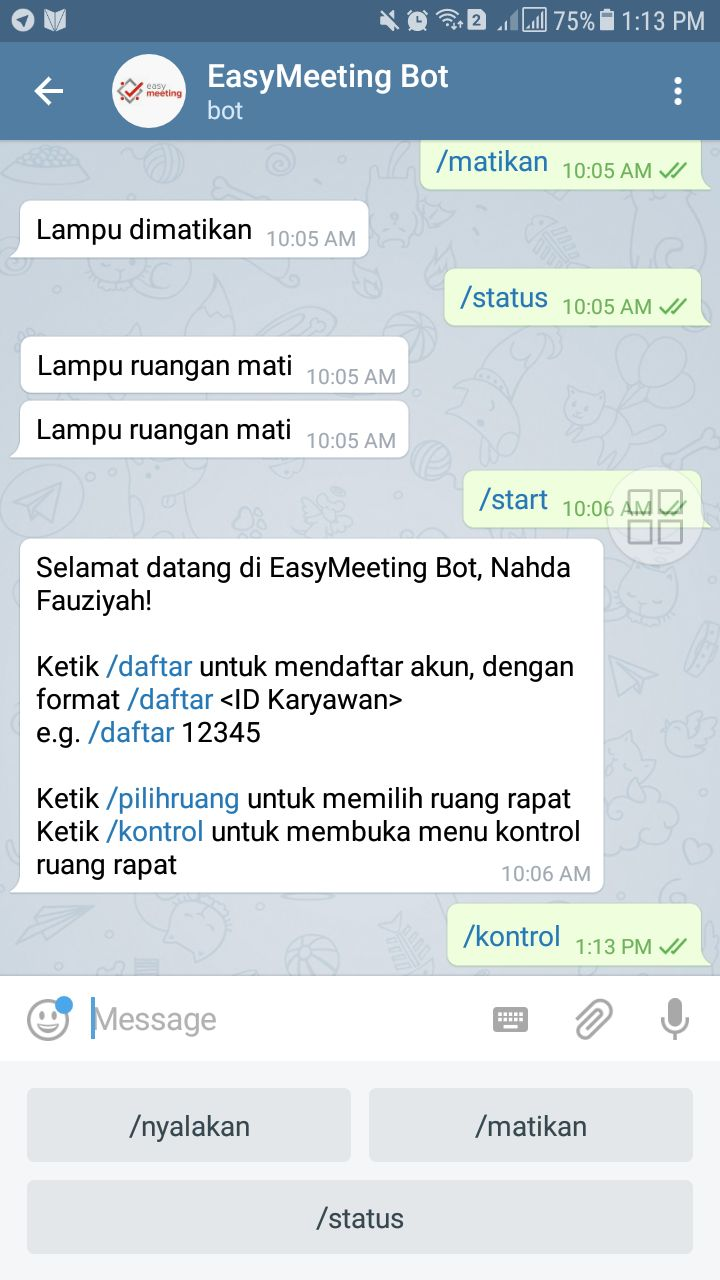
\includegraphics[width=3.5cm]{bab6/img/kontrol.jpeg}
	}
	\caption{Mengirimkan Perintah "/kontrol"}
	\label{figure:kontrol}
\end{figure}
\begin{figure}[H]
	\centerline {
		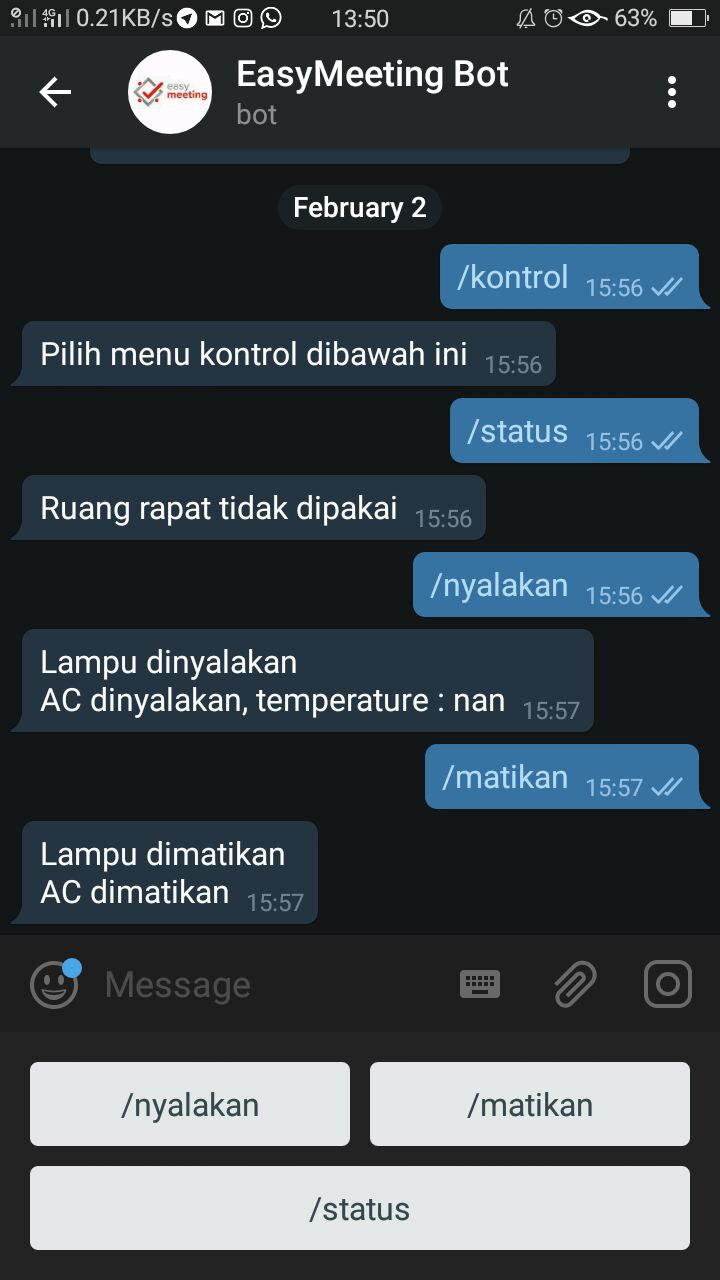
\includegraphics[width=3.5cm]{bab6/img/jalankan.jpeg}
	}
	\caption{Mengirimkan Perintah "/nyalakan", "/matikan", dan "/status"}
	\label{figure:jalankan}
\end{figure}

\begin{table}[h!]
	\centering
	\begin{tabular}{|p{6cm}|p{4cm}|}
		\hline
		\textbf{Tugas} & \textbf{Hasil}\\ \hline
		Sistem dapat menyalakan dan memadamkan lampu & Terpenuhi\\ \hline
		Sistem dapat menyalakan dan memadamkan AC & Terpenuhi\\ \hline
		Sistem dapat menampilkan status kondisi lampu dan AC ruangan & Terpenuhi\\ \hline
		Sistem dapat menampilkan suhu ruangan & Terpenuhi\\ \hline
		Sistem dapat diimplementasikan dengan menggunakan WSO2 IoT Server & Tidak Terpenuhi\\ \hline
	\end{tabular}\caption{Hasil Pengujian}
	\label{tab:hasil_pengujian}
\end{table}

Berdasarkan hasil pengujian yang telah dilakukan, dapat disimpulkan bahwa sistem easymeeting memenuhi kriteria yang disebutkan pada sub-bab sebelumnya, tetapi belum dapat diuji terhadap WSO2 IoT Server pada PT. Telekomunikasi Indonesia. Tabel \ref{tab:hasil_pengujian} adalah hasil pengujian pada sistem easymeeting.

\vspace{4 cm}
\textcolor{white}{..}